\documentclass[10pt,a4paper,twocolumn,twoside]{article}
\usepackage[utf8]{inputenc}
\usepackage[catalan]{babel}
\usepackage{multicol}
\usepackage{graphicx}
\usepackage{fancyhdr}
\usepackage{times}
\usepackage{titlesec}
\usepackage{url}
\usepackage{multirow}
\usepackage{lettrine}
\usepackage[top=2cm, bottom=1.5cm, left=2cm, right=2cm]{geometry}
\usepackage[figurename=Fig.,tablename=TAULA]{caption}
\usepackage{mathtools}
\captionsetup[table]{textfont=sc}

\author{\LARGE\sffamily Miquel Freixes Faya}
\title{\Huge{\sffamily Anàlisis de la relació entre les emisions de Co2 i l'augment de la temperatura, mitjançant tècniques i tecnologies de Big Data. 2n Informe de Seguiment}}
\date{}

\newcommand\blfootnote[1]{%
  \begingroup
  \renewcommand\thefootnote{}\footnote{#1}%
  \addtocounter{footnote}{-1}%
  \endgroup
}

%
%\large\bfseries\sffamily
\titleformat{\section}
{\large\sffamily\scshape\bfseries}
{\textbf{\thesection}}{1em}{}

\begin{document}

\fancyhead[LO]{\scriptsize MIQUEL FREIXES FAYA: TÍTOL DEL TREBALL}
\fancyhead[RO]{\thepage}
\fancyhead[LE]{\thepage}
\fancyhead[RE]{\scriptsize EE/UAB TFG INFORMÀTICA: TÍTOL (ABREUJAT SI ÉS MOLT LLARG)}

\fancyfoot[CO,CE]{}

\fancypagestyle{primerapagina}
{
   \fancyhf{}
   \fancyhead[L]{\scriptsize TFG EN ENGINYERIA INFORMÀTICA, ESCOLA D'ENGINYERIA (EE), UNIVERSITAT AUTÒNOMA DE BARCELONA (UAB)}
   \fancyfoot[C]{\scriptsize ``Febrer'' de 2019, Escola d'Enginyeria (UAB)}
}

%\lhead{\thepage}
%\chead{}
%\rhead{\tiny EE/UAB TFG INFORMÀTICA: TÍTOL (ABREUJAT SI ÉS MOLT LLARG)}
%\lhead{ EE/UAB \thepage}
%\lfoot{}
%\cfoot{\tiny{February 2015, Escola d'Enginyeria (UAB)}}
%\rfoot{}
\renewcommand{\headrulewidth}{0pt}
\renewcommand{\footrulewidth}{0pt}
\pagestyle{fancy}

%\thispagestyle{myheadings}
\twocolumn[\begin{@twocolumnfalse}

%\vspace*{-1cm}{\scriptsize TFG EN ENGINYERIA INFORMÀTICA, ESCOLA D'ENGINYERIA (EE), UNIVERSITAT AUTÒNOMA DE BARCELONA (UAB)}

\maketitle

\thispagestyle{primerapagina}
%\twocolumn[\begin{@twocolumnfalse}
%\maketitle
%\begin{abstract}
\begin{center}

{\vrule depth 0pt height 0.5pt width 4cm\hspace{7.5pt}%
\raisebox{-3.5pt}{\fontfamily{pzd}\fontencoding{U}\fontseries{m}\fontshape{n}\fontsize{11}{12}\selectfont\char70}%
\hspace{7.5pt}\vrule depth 0pt height 0.5pt width 4cm\relax}

\end{center}

\bigskip
%\end{abstract}
\end{@twocolumnfalse}]

\blfootnote{$\bullet$ E-mail de contacte: m.freixes.faya@gmail.com}
\blfootnote{$\bullet$ Menció realitzada: Tecnologies de la Informació}
\blfootnote{$\bullet$ Treball tutoritzat per: Jordi Casas Roma (departament)}
\blfootnote{$\bullet$ Curs 2018/19}

\section{Evolució de la Planificació}
\lettrine[lines=3]{L}{a} planificació està seguint el que es va programar a l'inici del treball, però amb les modificacions que es van fer en el segon informe de seguiment. Actualment el treball està en la fase final on només falta acabar de perfeccionar resultats, potser la planificació s'acabi allargant més gràcies al fet que, un cop acordat amb el tutor, s'hagi decidit d'analitzar les xarxes neuronals més simples. Segurament també s'acabi afegint una anàlisi d'un altre algorisme basat en model com el lineal. Això és degut als mals resultats que ha donat l'algorisme de Support Vector Machines i també a causa del fet que, com ja s'havia planificat amb temps per possibles imprevistos o millores i no s'ha produït cap destacable, hi ha suficient temps per fer provar nous algorismes. Per tant es pot considerar que la planificació feta per complir els objectius inicials s'està seguint, no obstant això, en ampliar el nombre d'algorismes a comparar, ha augmentat el seu temps fins a l'entrega de la proposta de l'informe final.
\section{ Evolució de la Metodologia}
La metodologia s'està seguint de la mateixa forma que a l'informe anterior. S'està pujant al GitHub tots els canvis i modificacions que es van fent al llarg del treball [1]. No obstant això, al mateix temps que en la fase anterior s'utilitzava el repositori de DataBricks, en aquesta fase sí que s'utilitza GitHub, ja que el programa Jupyter no té un repositori com a tal. També se segueix utilitzant Kanban per organitzar les tasques que han anat apareixent al llarg de la fase, com es va dir anteriorment, es divideix per fases per simplificar el procés i poder prioritzar amb més detall les tasques. 
\section{Entrenament i avaluació dels algorismes}
Aquesta fase s'ha centrat a provar diferents algorismes de regressió de la llibreria Scikit-Learn per determinar quin pot aconseguir predir millor les temperatures segons les diferents emissions de gasos hivernacle. Abans de començar a entrenar algorismes, calia entendre bé quines eren les dades que formaven el \textit{DataSet}. Encara que en la fase anterior s'hagués creat el \textit{DataSet} calia veure si les temperatures variaven molt entre diferents anys, i si era una variació constant o amb una certa aleatorietat. Per fer-ho s'ha tret uns gràfics amb la temperatura de Gener al llarg de diversos anys. En la figura 1 es pot veure les temperatures del mes de Gener a Austria. És visible que la temperatura no presenta cap patró que pugui facilitar l'obtenció de bons resultats, ja que hi ha variacions d'1 o 2 graus però també de 4 o 5 en alguns anys.
\begin{figure}[!h]
\centering
	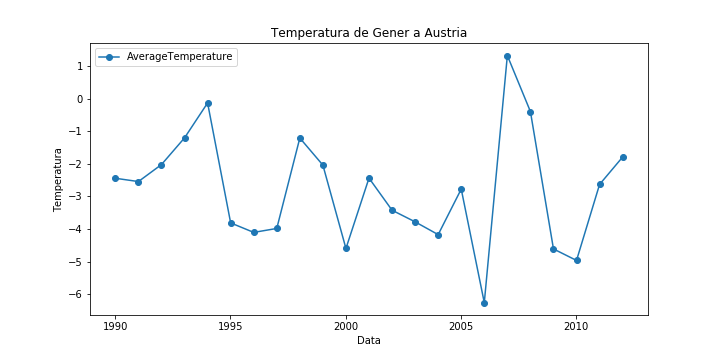
\includegraphics[width=0.5\textwidth]{img/tempAustria}
	\caption{Temperatures }
	\label{fig-tempAustria}
\end{figure}
A més d'analitzar el \textit{DataSet} també ha estat necessari passar els països a dades numèriques, ja que Scikit-Learn no permet \textit{Strings} per entrenar els seus algorismes [2]. Aquesta acció s'havia de fer d'una manera que no convertís les variables en categòriques, és a dir, que l'algorisme no entengués que ser d'un país o d'un altre tenia una relació numèrica. Per fer-ho s'ha utilitzat un mètode de la mateixa llibreria de SciKit-Learn que transforma els \textit{String} en variables binàries, per tant si és d'un país, serà un 1 i si no ho és, serà 0.

Un cop sabent que el \textit{DataSet} era adequat per fer aquestes anàlisis, s'ha començat a escollir i entrenar diversos algorismes de regressió. Els algorismes de regressió són tasques d'aprenentatge inductiu [2]. Es diferencien en les tasques de classificació a causa del fet que en la regressió es prediuen valors numèrics, en canvi en la classificació es prediuen etiquetes de classe. La tasca de regressió consisteix en l'assignació de variables sobre un domini donat, aquestes variables estan descrites per atributs discrets. A partir d'aquest conjunt de dades, els algorismes de regressió assignen valors numèrics a instàncies d'aquest domini amb la finalitat d'aconseguir una aproximació a partir de valors que es donen~[3].

Dins de la regressió s'ha decidit agafar un conjunt de mètodes que es considerin dins de l'estat de l'art actual en temes de \textit{Machine Learning} (ML).
\begin{itemize}
\item \textbf{Arbres de Decisió:} Els arbres de decisió són models predictius no linears que serveixen per fer tasques de regressió i tasques de classificació. La idea és simple, si es vol predir una classe o resposta Y a partir d'entrades X cal fer créixer un arbre binari. En els nodes d'aquest arbre binari s'aplica un test sobre l'input que es consideri més rellevant, per exemple en la figura 2 es comença preguntant sobre la contaminació de CO$_2$. En aquest test es fa una pregunta binària de si o no, si la resposta és si es passarà al fill de la dreta, si la resposta és no, es passarà al fill de l'esquerra. A partir d'aquí es van fent tests en cada un dels nodes, l'input que s'agafa per formular la pregunta pot variar segons les dades que s'estiguin treballant. Com es mostra a la figura 2 si s'envà cap a l'esquerra, es passa a testejar l'input de les emissions de CH$_4$. A la figura també es pot observar com les prediccions sobre quina és la temperatura final s'acaben fent en arribar a les fulles de l'arbre. Aquestes prediccions vénen donades pel conjunt de totes les preguntes que s'han anat formulant en els seus antecessors [4].
\begin{figure}[!h]
\centering
	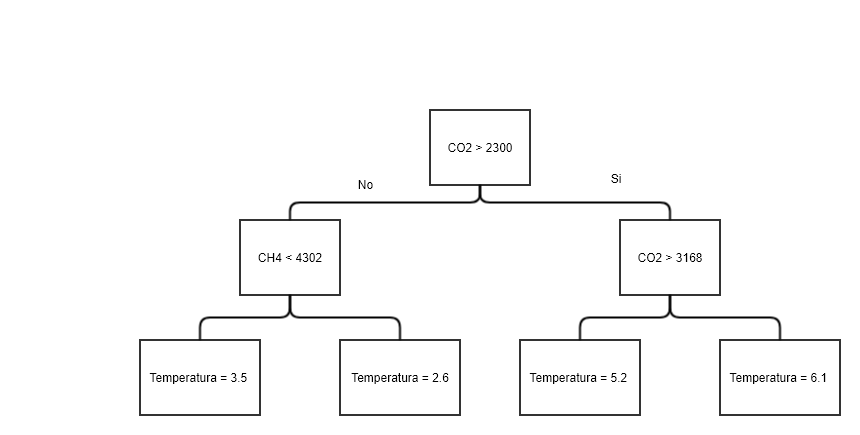
\includegraphics[width=0.5\textwidth]{img/arbreDecisioSimple}
	\caption{Arbre de Decisió Bàsic}
	\label{fig-DecisionTree}
\end{figure}
Quan hi ha molts inputs a l'hora d'entrenar l'arbre de decisió, el mateix arbre ha d'escollir quin paràmetre dels inputs cal avaluar primer. Una mala elecció d'aquest input pot comportar que es comenci a fer comprovacions innecessàries, causant un impacte negatiu en l'eficiència de l'entrenament. L'arbre de decisió fa aquesta elecció a partir d'una recerca mitjançant la força bruta, en aquesta s'intenta buscar quina és la pregunta que pot aportar més informació de cara als següents nodes. Aquesta decisió la fa en cada un dels nodes i va variant fins a arribar a una fulla. Si en aquesta recerca es trobessin dues preguntes sobre dos inputs, que donen la mateixa quantitat d'informació, l'arbre escull una arbitràriament [4].

Per acabar, els arbres de decisions tenen molts paràmetres editables com la seva longitud màxima, el nombre màxim de fulles, el mínim nombre de paràmetres per considerar el node com una fulla... La majoria d'aquests paràmetres limiten el creixement de l'arbre, ja que per defecte creix fins a fer totes les preguntes possibles. Aquests paràmetres són molt importants en l'obtenció de bons resultats, parar el creixement d'un arbre, en una profunditat equivocada, pot fer que l'arbre acabi descartant gran part d'informació, ja que no tots els nodes donen la mateixa quantitat d'informació a l'arbre[4].
\item \textbf{Support Vector Machines:}
Support Vector Machines o SVM és un mètode d'aprenentatge supervisat que es poden utilitzar per a la classificació i la regressió. Aquest té com a objectiu principal definir una funció f(x) que tingui com a molt una desviació o error per sota d'un límit establert en la creació del mètode. Per exemple, si s'estableix un error igual a 1, es descartaran tots els objectius amb un error superior a 1, i es consideraran tots els que tinguin un valor inferior. El SVM treballa amb productes sobre punts dins de dimensions definides, això troba les familiaritats entre dos vectors. SVM tenen un paràmetre essencial anomenat kernel, bàsicament són un conjunt de fórmules matemàtiques que defineixen com es processarà les dades que entren com a inputs. Els kernels són els encarregats de modificar el producte de punts establert pel SVM i adaptar-lo al seu espai. Per defecte el SVM té com a kernel el lineal, que limita el producte de punts original en dues dimensions. Si en lloc del lineal s'utilitzes un kernel com el polinòmic, aquest espai acceptaria també combinacions polinòmiques fins a certs graus, aconseguint fer paràboles [5]. A més d'aquests dos, hi ha un de molt utilitzat anomenat Radial Basis Function o RBF. Aquest utilitza un espai limitat per distribucions Gaussianes, en la majoria d'ocasions aquest kernel és el que pot arribar a obtenir els millors resultats [6].
\item \textbf{Random Forest:}
El Random Forest és un dels mètodes de ML que s'està utilitzant més en l'actualitat, com els altres dos, es pot utilitzar tant per classificació com per regressió. La idea principal del Random Forest és la combinació de molts arbres de decisió iguals relacionats entre ells, això ho fa gràcies al fet que es basa en la idea que la combinació de molts algoritmes iguals aconsegueix millors resultats que un de sol molt potent. Com es pot veure a la figura 3, que representa un Random Forest amb dos arbres, el mètode crea dos arbres de decisió i després combina els resultats de cada un d'ells mitjançant el Bagging Method o un altre algoritme segons la implementació que s'esculli [7].

Aquest mètode té pràcticament els mateixos paràmetres que un arbre de decisió però amb petites diferències que optimitzen cada una de les decisions preses per l'arbre. Com s'ha dit anteriorment els arbres necessiten escollir quina pregunta s'ha de fer en cada node per aconseguir informació a l'hora de separar les variables, el Random Forest modifica aquesta elecció. En lloc d'escollir la millor opció de totes agafa un subconjunt dels inputs que arriben al node i escull la millor dins d'aquest subconjunt [8]. El Random Forest permet editar molts paràmetres entre els quals destaquen el nombre d'arbres de decisió que es combinaran, el nombre d'inputs que s'inclouran en el subconjunt aleatori, també es pot escollir tots els paràmetres per editar els arbres de decisió o fins i tot l'algorisme que combinarà els seus resultats.
\begin{figure}[!h]
\centering
	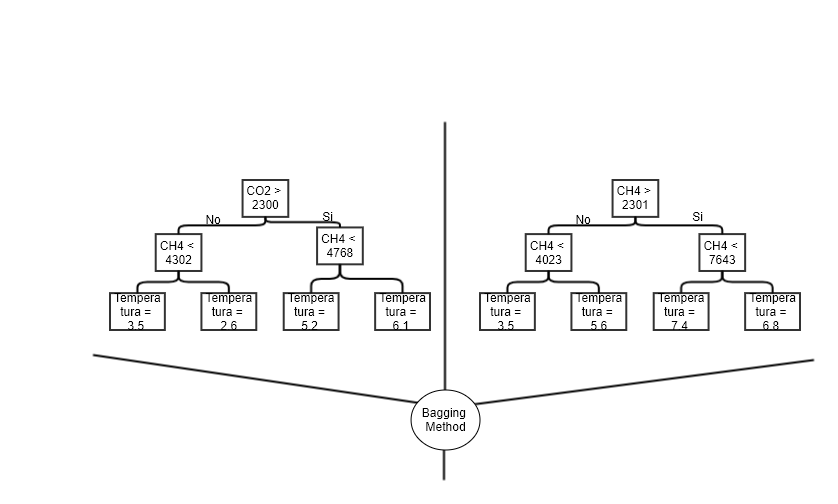
\includegraphics[width=0.5\textwidth]{img/randomForest}
	\caption{Random Forest amb 2 arbres}
	\label{fig-RandomForest}
\end{figure}
\end{itemize}
D'aquests algorismes s'ha fet un entrenament amb els paràmetres per defecte marcats per la llibreria de Scikit-Learn i després s'ha utilitzat dues tècniques, molt utilitzades en l'àmbit del ML per trobar el conjunt de paràmetres més òptim per cada algorisme. Aquestes tècniques tenen com a objectiu esprémer al màxim els algorismes i aconseguir l'aproximació més precisa de la temperatura. Aquestes tècniques han estat:
 \begin{itemize}
\item \textbf{Grid SearchCV:} )Implementa una recerca exhaustiva dels paràmetres editables d'un mètode de predicció. Un cop fet aquest anàlisis entrena l'algorisme amb la millor combinació de paràmetres que ha trobat. Amb cada una de les combinacions fa 3 iteracions i després utilitza una fórmula per avaluar el resultat obtingut, aquest pot ser el Mean Absolute Error o MAE, Mean Squared Error [9]... Les iteracions dels paràmetres les fa en ordre ascendent, comença pels paràmetres més petits i va augmentant-los fins al límit que se l'hi ha establert.
\item \textbf{Randomized SearchCV:} És un mètode molt semblant al Grid Search. També fa una recerca sobre els millors paràmetres que aconsegueixin treure el millor resultat del mètode. La principal diferència és que en lloc de fer-ho de forma iterativa i ascendent ho fa de forma iterativa però aleatòriament. Això permet que es puguin provar valors molt elevats sense necessitat de què la recerca augmenti exponencialment el temps necessari per acabar [10].
\end{itemize}
\section{Resultats i conclusions provisionals}
Per aconseguir els resultats s'ha hagut d'aplicar tant el Grid Search com el Randomized Search amb les mateixes iteracions als tres algorismes escollits, amb els mateixos conjunts de dades per cada un d'ells. En tots els casos els millors resultats els ha donat la tècnica de Randomized Search. Això s'ha donat a causa del fet que la tècnica pot editar paràmetres molt més grans i diversos. El Grid Search no pot fer el mateix pel fet que el Randomized utilitza iteracions de valors aleatoris, dins d'un rang molt més gran de valors. En canvi, el Grid Search està limitat a anar fent proves seqüencialment, començant pels valors més petits i fins a arribar al màxim del rang que s'ha establert. Al cap i a la fi el Grid Search està limitat per la quantitat elevada de càlculs que necessita fer. Per exemple, ficant el mateix nombre de variables, amb el mateix rang de valors en cada una d'elles, per arribar al valor màxim el Grid Search ha de fer X iteracions prèvies (on X pot ser un número molt elevat d'iteracions), en canvi el Randomized ho pot fer a la primera sense passar per totes les anteriors.

Amb el Randomized s'ha aconseguit els millors resultats per cada un dels algorismes aplicats. Com es pot veure a la figura 4 l'algorisme que ha aconseguit aproximar-se més als valors originals ha estat el Random Forest, en canvi el pitjor ha estat l'algorisme de les Support Vector Machine.
\begin{figure}[!h]
\centering
	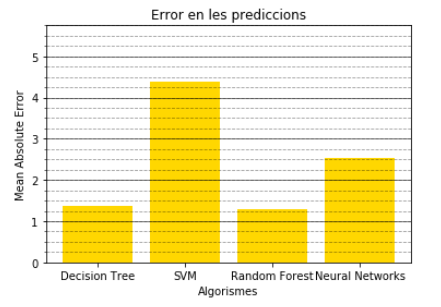
\includegraphics[width=0.5\textwidth]{img/comparacioMetricsAlgs}
	\caption{MAE dels mètodes}
	\label{fig-Metrics}
\end{figure}
Veient les comparacions amb les temperatures reals de la figura 5 es pot veure com les SVM no s'està adaptant bé a cap canvi de temperatura, bàsicament es manté constant en 10 graus excepte en tres ocasions que sembla que intenta aproximar-se més a la temperatura real. Això pot ser degut a l'elecció de kernel o del paràmetre C. Tal com es mostra a la gràfica les SVM no estan tenint un resultat gens esperat, els resultats poden venir donats també per una incompatibilitat entre el conjunt de dades i l'algorisme. Els altres dos algorismes si que s'aproximen molt en les seves prediccions, fallen entre 1 i 1.5 graus en la majoria de temperatures.

Aquests resultats són molt bons a causa del fet que l'error és bastant baix, considerant que la temperatura varia d'un any per l'altre entre 2 i 4 graus. No obstant això, els dos mètodes tenen un comportament una mica diferent a l'hora de fer prediccions. El Random Forest manté bastant la constància amb les temperatures que no varien massa, en canvi sí que falla bastant quan hi ha un canvi brusc de temperatura. Per l'altra banda els Decision Tree fallen en la gran majoria de prediccions però amb un error baix en tots ells, això fa que el MAE d'ambdós sigui molt semblant, encara que el Random Forest acabi tenint un més baix.

Com a idees per continuar aquest TFG es podria fer la mateixa anàlisi de les dades però en un àmbit mundial en lloc d'Europeu. Segurament els resultats siguin encara millors gràcies a un nombre més gran de dades a analitzar. Una altra possible continuació pot ser l'increment d'algorismes de ML amb els que analitzar les dades, ja que en aquest treball s'han obviat alguns mètodes com les Xarxes Neuronals, que actualment estan donant resultats molt impressionants en l'àmbit del ML i del Deep Learning.
\begin{figure}[!h]
\centering
	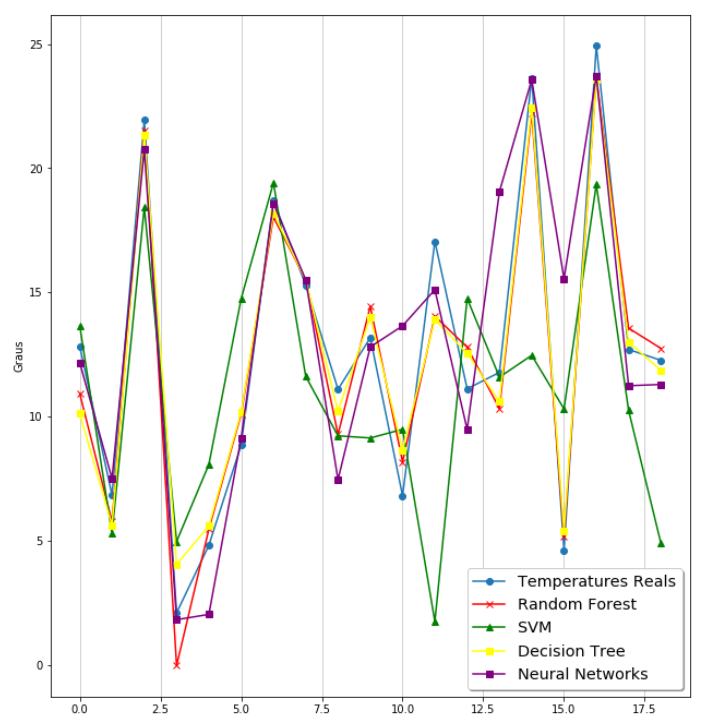
\includegraphics[width=0.5\textwidth]{img/comparacioAlgs}
	\caption{Comportament dels mètodes}
	\label{fig-temps}
\end{figure}

\begin{thebibliography}{11}
\bibitem{1}
Miquel Freixes, ``Treball de Fi de Grau de Miquel Freixes". \textit{GitHub}. [En línia]. Disponible a: \url{ https://github.com/miky96/TFG}. [Accedit Novembre 10, 2018].
\bibitem{2}
``Encoding Categorical Features", \textit{Scikit-Learn}. [En línia]. Disponible a:\url{https://scikit-learn.org/stable/modules/preprocessing.html#encoding-categorical-features}. [Accedit Desembre 22, 2018].
\bibitem{3}
F.Julbe, \textit{Anàlisi de dades massives: Tècniques fonamentals}. Barcelona, UOC. Pàgines: 43-45.
\bibitem{4}
R. Tibshirani, \textit{Classication and Regression Trees}. Machine Learning Department, Carnegie Mellon University. 2009.
\bibitem{5}
Alex J. Smola, B. Schölkopf, \textit{A tutorial on support vector regression}. RSISE, Australian National University. 2003.
\bibitem{6}
\url{https://data-flair.training/blogs/svm-kernel-functions/}
\bibitem{7}
``Kernel Functions-Introduction to SVM Kernel \& Examples", \textit{Data Flair}. [En línia]. Disponible a:\url{https://towardsdatascience.com/the-random-forest-algorithm-d457d499ffcd}. [Accedit Desembre 22, 2018].
\bibitem{8}
L. Breiman, \textit{Random Forests}. Statistics Department, University of California Berkeley. 2001.
\bibitem{9}
``Grid Search CV", \textit{Scikit-Learn}. [En línia]. Disponible a:\url{https://scikit-learn.org/0.15/modules/generated/sklearn.grid_search.Grid SearchCV.html#sklearn.grid_search.Grid SearchCV}. [Accedit Desembre 22, 2018].
\bibitem{10}
``Randomized Search CV", \textit{Scikit-Learn}. [En línia]. Disponible a:\url{https://scikit-learn.org/stable/modules/generated/sklearn.model_selection.Randomized SearchCV.html}. [Accedit Desembre 22, 2018].

\end{thebibliography}
\clearpage
\section{Annex}
 \begin{itemize}
\item \textbf{Temperatures Espanya:}
\begin{figure}[!h]
\centering
	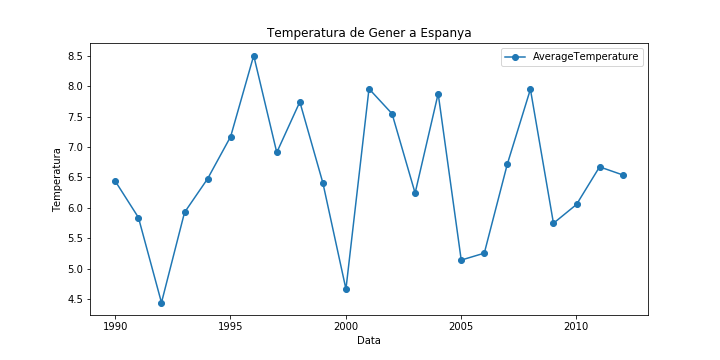
\includegraphics[width=1\textwidth]{img/tempSpain}
	\caption{Temperatura a Espanya}
	\label{fig-tempSpain}
\end{figure}
\item \textbf{Temperatures Alemanya:}
\begin{figure}[!h]
\centering
	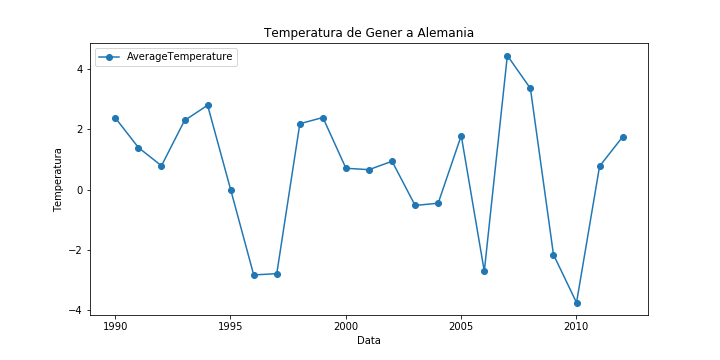
\includegraphics[width=1\textwidth]{img/tempGermany}
	\caption{Temperatura a Alemanya}
	\label{fig-tempGerm}
\end{figure}
\end{itemize}
\end{document}

